\section{Routing}

\begin{description}
		\item[Proactive routing] Pre-calculated (static or dynamic) routing tables, eg OLSR
		\item[Reactive routing] Route establishment on-demand, eg AODV
\end{description}

\begin{itemize}
		\item For WSNs, routing protocols must be scalable, work locally, be
				robust, and have a low overhead.
		\item Use WSN-specific routing metrics such as energy, number of hops,
				QoS, link quality
\end{itemize}

\subsection{Expected transmission count}

Loss probability in forward and reverse direction $p_f, p_r$. Then: 
\begin{align*}
		p & = 1 - (1 - p_f) \cdot (1 - p_r) && \text{Probability of non-successful transmission} \\
		s(k) & = p^{k-1} \cdot (1 - p) && \text{Probability for successful delivery after k attempts} \\
		ETX & = \sum_{k = 1}^{\infty} k \cdot s(k) = \frac{1}{1-p} && \text{Expected transmission count}
\end{align*}

\subsection{Routing protocols}

\subsubsection{Flat network, Ad-Hoc On-Demand Distance Vector Routing, AODV}

\begin{itemize}
		\item When no valid route known, node generates route request (RREQ)
				containing last known sequence number and IP of destination
		\item When RREQ received, node a) generates reverse routing for RREQ's
				source, and b) responds to RREQ with route reply (RREP) if
				valid route known.  Otherwise broadcasts it. Repeated RREQ in
				short amount of time ignored.
		\item RREP (by destination or intermediary node) arrives back at
				source. All nodes which have received it use the information
				(if newer than what is known) to update their routing tables.
		\item If route invalid, route error (RERR) sent by node detecting failure
\end{itemize}

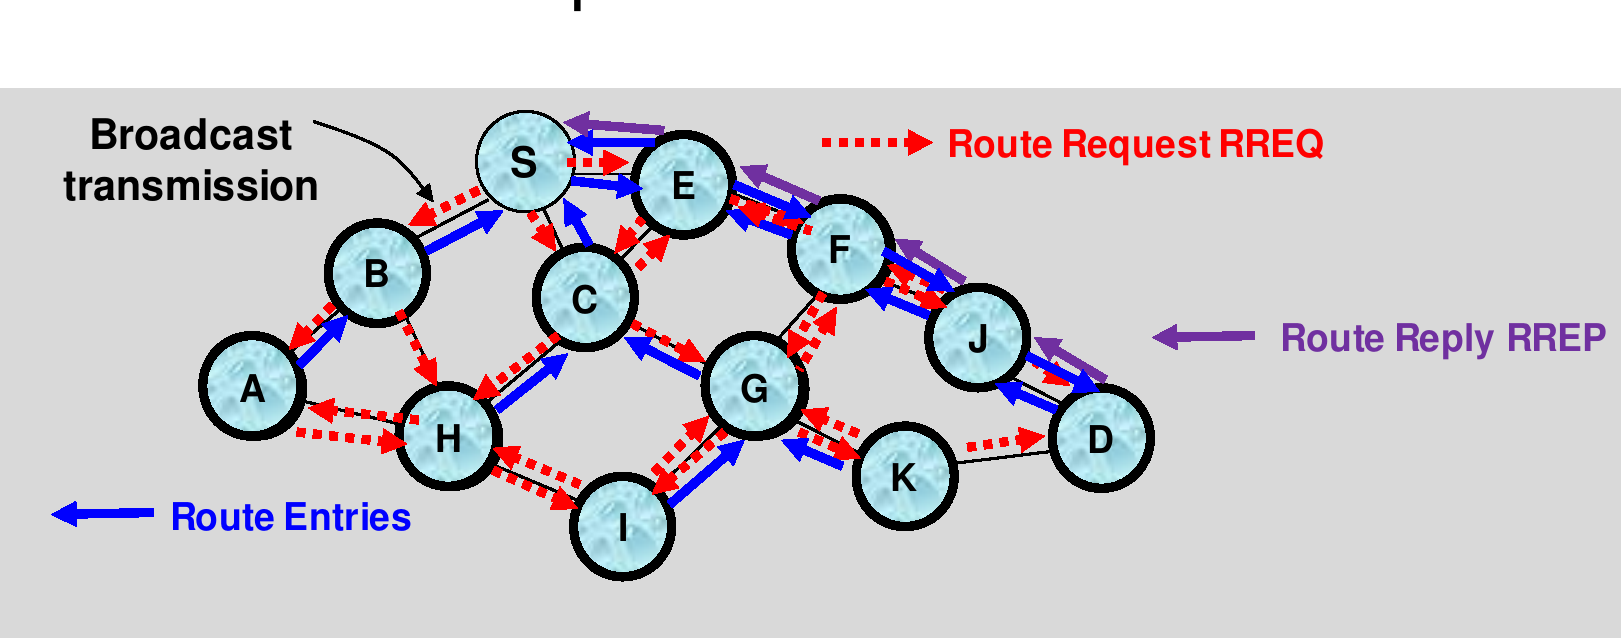
\includegraphics[width=0.5\textwidth]{08_aodv}

\subsubsection{Data-centric}

Idea: No addressing of nodes by address, instead forward packets based on
contained data.

\paragraph{Directed diffusion}

\begin{itemize}
		\item Nodes specify attribute/value pairs they are interested in
		\item Interest propagated and periodically refreshed
		\item Gradients define, based on interests, which way data matching
				interest should flow. Interest can specify data rate and
				liefetime.
		\item Node generating data sends only as much as its outgoing gradients
				permit, along the gradients. Receiving nodes forward along
				their known gradients, dropping recently received packets to
				prevent loops.
		\item Sinks receiving data of interest reinforce gradient by e.g.
				increasing data rate. Nodes which receive a reinforcement must
				also reinforce at least one neighbour.
		\item Convergence to few paths per sink and interest.
\end{itemize}

\subsubsection{Geographic routing}

Idea: Nodes known their geographic location and immediat neighbours. Routing
destination specified as location or geographic region.

\paragraph{Greedy perimeter stateless routing}

\begin{itemize}
		\item Greedy forwarding to closest neighbour to destination
		\item If greedy not possible, switch to recovery mode \textbf{until
				closer to destination than where recovery mode was entered}. In
				recovery mode: 1) right-hand-rule (pick next node
				counterclockwise from inbound edge) and perimeter routing (do
				not intersect source - destination line)
\end{itemize}

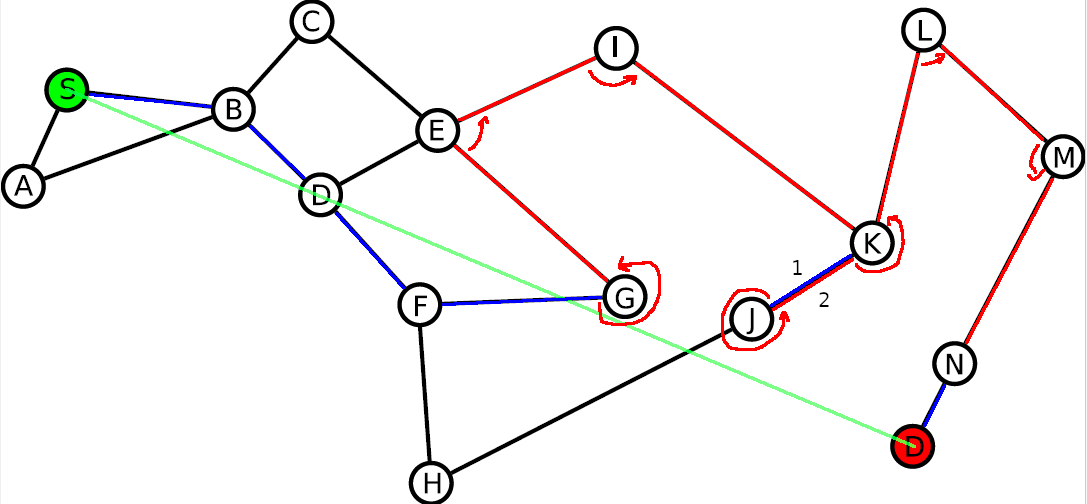
\includegraphics[width=0.5\textwidth]{08_gpsr}

\paragraph{Geographic hash tables}

\begin{itemize}
		\item Hashing of a key (contents of data) into geographic coordinates.
		\item Data stored on sensor node (``home node'') closest to hash of its key
		\item Allows all data related to one event (eg a forest fire) to be stored on one node
		\item Home node determined by GPSR. First greedy routing towards
				destination coordinates. At closest node (which does not yet
				know it is closest!) permieter routing is entered and 'circles
				around' the coordinate. Once node receives packet a second
				time, it knows it is home node.
\end{itemize}

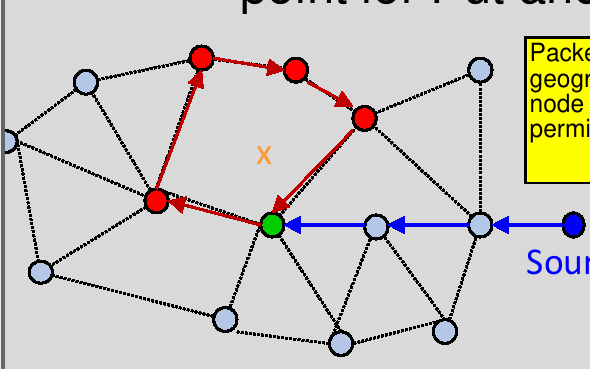
\includegraphics[width=0.5\textwidth]{08_ght}

\subsubsection{Hierarchical routing}

\begin{itemize}
		\item Cluster formation, with one cluster lead each
		\item Sensor nodes forward data to cluster lead which aggregates, and
				forwards to sink via other cluster leads
\end{itemize}

\paragraph{Two-tier data dissemination}

\begin{itemize}
		\item Nodes aware of own location
		\item Source sends out event, greedy forwarding towards destination
		\item Grid construction: Source defines cell size, located at crossint
				point of two grid lines. Nodes closest to adjacent 4 crossing
				points become cluster leaders, which propagate this to nodes
				nearest to their crossing points.
		\item Then, greedy forwarding can move along so-defined leaders (close
				to crossing points)
\end{itemize}

\subsection{IPv6 in WSNs}

Problems: Large overhead (IPv6 header of 40 bytes), too large MTU (1280 bytes)
for error-prone networks, devices unable to process complex routing protocols,
unstable network.

\subsubsection{6LowPAN Routing}

Low-power routing options:
\begin{description}
		\item[Mesh under] Link-layer forwarding, no IP routing. Broadcast link has to be emulated
		\item[Route over] Routing at IP layer, each node is IP router
		\item[Header compression] Compression of certain fields of IPv6 header where data can be inferred from other layers, or generic compression using e.g. LZ77.
		\item[Fragmentation] Fragmentation on link-level allows smaller MTU
\end{description}

\subsubsection{RPL, Routing protocol for low-poer and lossy networks}

\begin{itemize}
		\item RPL forms multiple DODAG (destination-oriented DAG), with root
				being gateway into WSN. Nodes can have redundant paths.
		\item Nodes can store routes (in which case they can route themselves),
				or not store it (in which case the root will route)
		\item Periodic broadcast of routing information (DIO, DODAG information
				object) from root to leaf nodes
		\item DIO can be requested via DIS (DODAG information solicitation)
		\item DAO (destination advertisement option) can be sent from leaf
				nodes to root, with each intermediary adding its ID to it.
\end{itemize}

\subsubsection{IPv6 over TSCH}

\begin{itemize}
		\item Targets industrial applications
		\item Assumes network-wide synchronization and reliable channel
		\item Allows scheduling IPv6 packets for real-time requirements
		\item Functions as logical link control layer between 6LowPAN and TSCH MACH
		\item Defines distributed scheduling protocol, allowing upper layers to
				create schedules.
\end{itemize}

\subsubsection{IPv6 low-power wide area networks}

\begin{itemize}
		\item For end devices, radios, application servers, ...
		\item Problem again: Overhead, MTU
		\item Solution: Static context header compression, fragmentation and reassembly
\end{itemize}
